\chapter{Suites numériques}
\thispagestyle{fancy}

\begin{bhistoire}
	Dès l'Antiquité, Archimède de Syracuse (-287 ; -212), met en oeuvre une procédure itérative pour trouver une approximation du nombre $\pi$. Il encadre le cercle par des polygones inscrits et circonscrits possédant un nombre de côtés de plus en plus grand. Par ce procédé,
	Archimède donne naissance, sans le savoir, à la notion de suite numérique.\\
	Vers la fin du XVII$^\text{e}$ siècle, des méthodes semblables sont utilisées pour résoudre des équations de façon approchée pour des problèmes de longueurs, d'aires, ...\\
	Un formalisme plus rigoureux de la notion de suite n'apparaitra qu'au début du XIX$^\text{e}$ siècle avec le mathématicien français Augustin Louis Cauchy (1789 ;1857).
\end{bhistoire}


\section{généralités sur les suites numériques}

\subsection{Définition d'une suite numérique}

\begin{bexemplet}{Exemple d'introduction}
	On considère une liste de nombres formée par tous les nombres impairs rangés dans l'ordre croissant : $1,3,5,7, \ldots$\\
	On note $\left(u_{n}\right)$ l'ensemble des éléments de cette suite de nombres tel que :\\
	$u_{0}=1, u_{1}=3, u_{2}=5, u_{3}=7, \ldots$\\
	On a ainsi défini une suite numérique.\\
	On peut lui associer une fonction définie sur $\mathbb{N}$ par 
	$$u: \mathbb{N} \rightarrow \mathbb{R}$$
	$$\phantom{......................}n \mapsto u(n)=u_{n}$$
	
\end{bexemplet}

\begin{bdefi}
	\begin{itemDef}
		\item \phantom{$\dfrac{1}{3}$}\pointille[\textwidth-1cm]\\
		\phantom{$\dfrac{1}{3}$}\pointille[\textwidth-1cm]
		\item \phantom{$\dfrac{1}{3}$}\pointille[\textwidth-1cm]
	\end{itemDef}
\end{bdefi}

\subsection{Suite définie par une formule explicite}

\begin{bexemples}
	\begin{itemEx}
		\item Pour tout $n$ de $\mathbb{N}$, on donne : $u_{n}=2 n$ qui définit la suite des nombres pairs. Les premiers termes de cette suite sont donc :\\
		$u_{0}=2 \times 0=0$\\
		$u_{1}=2 \times 1=2$\\
		$u_{2}=2 \times 2=4$\\
		$u_{3}=2 \times 3=6$
		\item Pour tout $n$ de $\mathbb{N}$, on donne $: v_{n}=3 n^{2}-1$ Les premiers termes de cette suite sont donc :\\
		$v_{0}=3 \times 0^{2}-1=-1$\\
		$v_{l}=3 \times 1^{2}-1=2$\\
		$v_{2}=3 \times 2^{2}-1=11$\\
		$v_{3}=3 \times 3^{2}-1=26$
	\end{itemEx}
\end{bexemples}
\begin{bdefi}
	\phantom{$\dfrac{1}{3}$}\pointille[\textwidth-1cm]\\
	\phantom{$\dfrac{1}{3}$}\pointille[\textwidth-1cm]\\
	\phantom{$\dfrac{1}{3}$}\pointille[\textwidth-1cm]
\end{bdefi}

\subsection{Suite définie par une relation de récurrence}
\begin{bexemples}
	\begin{itemEx}
		\item On définit la suite $\left(v_{n}\right)$ par : $v_{0}=3$ et pour tout $n$ de $\mathbb{N}, v_{n+1}=4 v_{n}-6$ Les premiers termes de cette suite sont donc :\\
		$v_{0}=3$\\
		$v_{1}=4 v_{0}-6=4 \times 3-6=6$\\
		$v_{2}=4 v_{1}-6=4 \times 6-6=18$\\
		$v_{3}=4 v_{2}-6=4 \times 18-6=66$\\
		Contrairement à une suite définie par une formule explicite, il n'est pas possible, dans l'état, de calculer par exemple $v_{13}$ sans connaître $v_{12}$.\\
		\ \\
		Cependant il est possible d'écrire un algorithme avec Python :
		\begin{center}
			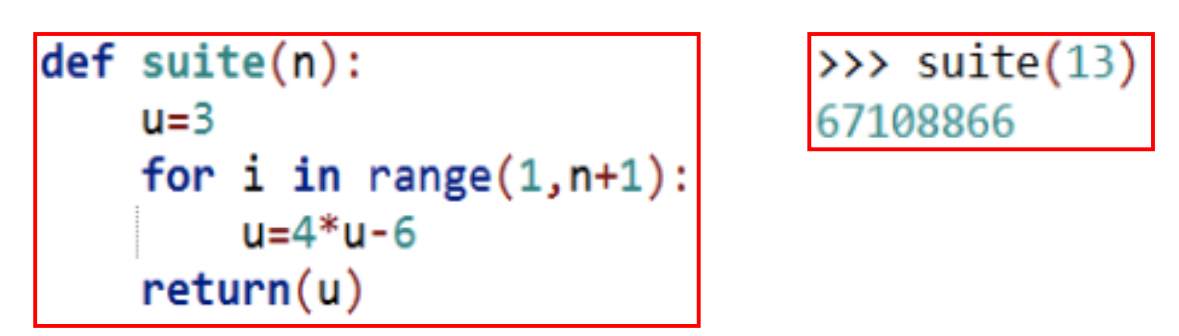
\includegraphics[scale=0.4]{1.08.00-Img01}
		\end{center}
	\end{itemEx}
\end{bexemples}
\begin{bdefi}
	\phantom{$\dfrac{1}{3}$}\pointille[\textwidth-1cm]\\
	\phantom{$\dfrac{1}{3}$}\pointille[\textwidth-1cm]\\
	\phantom{$\dfrac{1}{3}$}\pointille[\textwidth-1cm]
\end{bdefi}

\begin{brmq}
	Le mot \emph{récurrence} vient du latin \emph{recurrere} qui signifie "revenir en arrière".
\end{brmq}

\subsection{Représentation graphique d'une suite}

Dans un repère du plan, on représente une suite par un nuage de points de coordonnées $\left(n ; u_{n}\right) .$
\begin{bexemple}
	Pour tout $n$ de $\mathbb{N}$, on donne $: u_{n}=\dfrac{n^{2}}{2}-3$.\\
	On construit le tableau de valeurs avec les premiers termes de la suite :
	\begin{tabular}{|Xc|Xc|Xc|Xc|Xc|Xc|Xc|Xc|Xc|Xc|}
		\hline$n$ & 0 & 1 & 2 & 3 & 4 & 5 & 6 & 7 & 8 \\
		\hline$u_{n}$ & $-3$ & $-2,5$ & $-1$ & 1,5 & 5 & 9,5 & 15 & 21,5 & 29 \\
		\hline
	\end{tabular}\\
	Il est possible d'obtenir un nuage de points à l'aide d'un logiciel.
	\begin{center}
		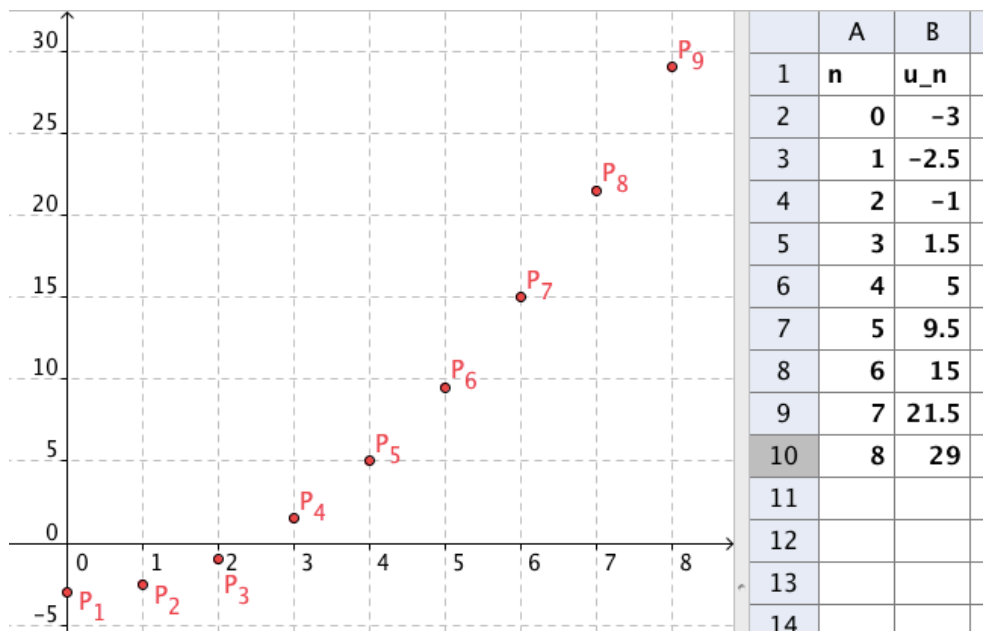
\includegraphics[scale=0.4]{1.08.00-Img03}
	\end{center}
	
\end{bexemple}


\section{Suites arithmétiques}

\subsection{Définition}

\begin{bexemple}
	Considérons une suite numérique $U_n$ où la différence entre un terme et son précédent reste constante et égale à 5.\\
	Si le premier terme est égal à 3, les premiers termes successifs sont :\\
	$U_0 = 3$,\\
	$U_1 = 8$,\\
	$U_2 = 13$,\\
	$U_3 = 18$.\\
	Une telle suite est appelée une suite arithmétique de raison 5 et de premier terme 3.
	La suite est donc définie par : $U_{n+1}=U_n+5$ et $U_0=3$.
\end{bexemple}

\begin{bdefi}
	\phantom{$\dfrac{1}{3}$}\pointille[\textwidth-1cm]\\
	\phantom{$\dfrac{1}{3}$}\pointille[\textwidth-1cm]\\
	\phantom{$\dfrac{1}{3}$}\pointille[\textwidth-1cm]
\end{bdefi}
\ \\
\begin{bmethodet}{Démontrer si une suite est arithmétique}
	1) La suite $U_n$ définie par : $U_n=7-9n$ est-elle arithmétique ?\\
	2) La suite $V_n$ définie par : $V_n=n^2+3$ est-elle arithmétique ?\\
	\\
	voir cahier
\end{bmethodet}

\begin{bprop}
	$U_n$ est une suite arithmétique de raison $r$ et de premier terme $U_0$.\\
	\phantom{$\dfrac{1}{3}$}\pointille[\textwidth-1cm]
\end{bprop}

\begin{bdemo}
	voir cahier.
\end{bdemo}

\begin{bmethodet}{Déterminer la raison et le premier terme d'une suite arithmétique}
	Considérons la suite arithmétique $U_n$ tel que $U_5=7$ et $U_9=19$.\\
	1) Déterminer la raison et le premier terme de la suite $U_n$.\\
	2) Exprimer $U_n$ en fonction de $n$.\\ 
	\\
	voir cahier
\end{bmethodet}

\subsection{Représentation graphique}

Les points de la représentation graphique d'une suite arithmétique sont alignés.

\begin{bexemple}
	On a représenté ci-dessous la suite de raison $–0,5$ et de premier terme $4$.
	\begin{center}
		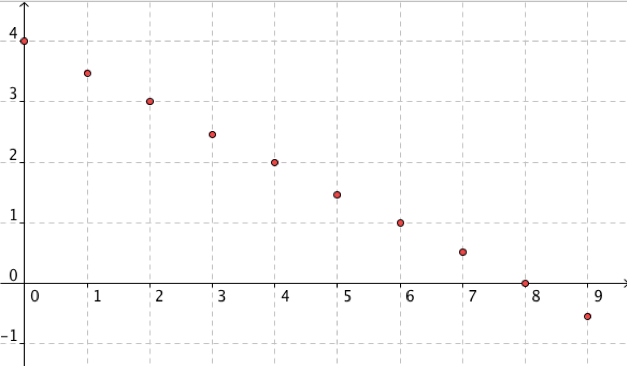
\includegraphics[scale=1]{01-07-01}
	\end{center}
\end{bexemple}

\section{Somme des termes consécutifs: suite arithmétique}

\begin{bprop}
	\phantom{$\dfrac{1}{3}$}\pointille[\textwidth-1cm]\\
\end{bprop}

\begin{brmq}
	Il s'agit de la somme des $n$ premiers termes d'une suite arithmétique de raison $1$ et de premier terme $1$
\end{brmq}

\begin{bdemo}
	voir cahier
\end{bdemo}

\begin{bmethodet}{Calculer la somme des termes d'une suite arithmétique}
	Calculer les sommes $S_1$ et $S_2$ suivantes :\\ 
	$S_1=1+2+3+...+348$\ \ \ \ \ \ \ \ \ \ \ \ \ \ \ \ \ \ \ \ \ \ \ $S_2=33+36+39+...+267$
	\\
	voir cahier
\end{bmethodet}

\section{Suites géométriques}

\subsection{Définition}

\begin{bexemple}
	Considérons une suite numérique $U_n$ où le rapport entre un terme et son précédent reste constant et égale à 2.\\
	Si le premier terme est égal à 5, les premiers termes successifs sont :\\
	$U_0 = 5$,\ \ \ 
	$U_1 = 10$,\ \ \ 
	$U_2 = 20$,\ \ \ 
	$U_3 = 40$.\\
	Une telle suite est appelée une suite géométrique de raison $2$ et de premier terme $5$.\\
	La suite est donc définie par : $U_{n+1}=2\times U_n$ et $U_0=5$. 
\end{bexemple}

\begin{bdefi}
	\phantom{$\dfrac{1}{3}$}\pointille[\textwidth-1cm]\\
	\phantom{$\dfrac{1}{3}$}\pointille[\textwidth-1cm]
\end{bdefi}

\begin{bmethodet}{Démontrer si une suite est géométrique}
	La suite $U_n$ définie par : $U_n=3\times 5^n$  est-elle géométrique ?
	\ \\
	voir cahier
\end{bmethodet}

\begin{bexemplet}{exemple concret}
	On place un capital de \EUR{500} sur un compte dont les intérêts annuels s'élèvent à $4\%$.
	Chaque année, le capital est multiplié par $1,04$.
	Ce capital suit une progression géométrique de raison $1,04$.\\
	
	On a ainsi :\\ 
	$U_1=1,04\times 500=520$\\		
	$U_2=1,04\times 520=540,80$\\
	$U_3=1,04\times 540,80=562,432$\\	
	De manière générale : $U_{n+1}=1,04\times U_n$ avec $U_0=500$\\ 
	On peut également exprimer $U_n$ en fonction de $n$ : $U_n= 500\times1,04^n$. 
\end{bexemplet}

\begin{propriete}
	$U_n$ est une suite géométrique de raison $q$ et de premier terme $U_0$.\\
	\phantom{$\dfrac{1}{3}$}\pointille[\textwidth-1cm]
\end{propriete}

\begin{bdemo}
	voir cahier
\end{bdemo}

\begin{bmethodet}{Déterminer la raison et le premier terme d'une suite géométrique}
	Considérons la suite géométrique $U_n$ tel que $U_4=8$ et $U_7=512$.\\
	Déterminer la raison et le premier terme de la suite $U_n$.\\
	\ \\
	voir cahier.
\end{bmethodet}

\subsection{Représentation graphique}

\begin{bexemple}
	La suite géométrique $U_n$ définie par $U_n=-4\times2^n$ est décroissante car le premier terme est négatif et la raison est supérieure à 1
	\begin{center}
		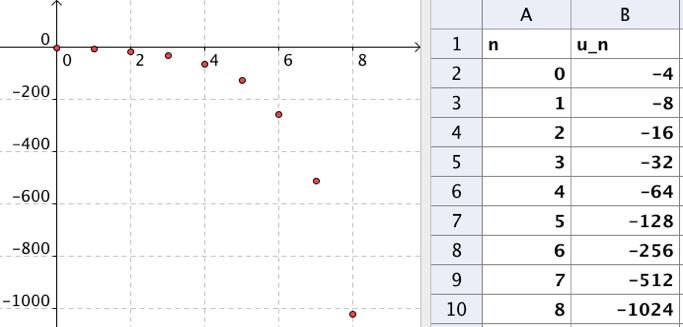
\includegraphics[scale=1]{01-07-03.png}
	\end{center}
	Remarque : Si la raison q est négative alors la suite géométrique n'est pas monotone.
\end{bexemple}
% \begin{center}
	%     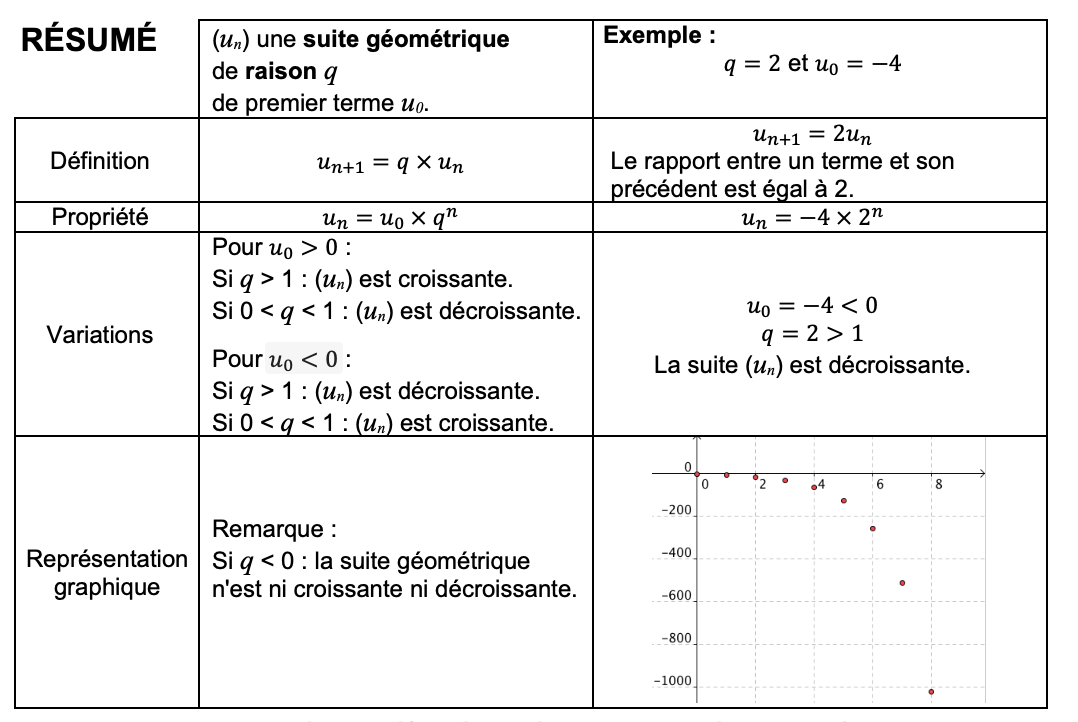
\includegraphics[scale=0.8]{01-07-04.png}
	% \end{center}

\section{Somme des termes consécutifs d'une suite géométrique}

\begin{bprop}
	$n$ est un entier naturel non nul et $q$ un réel différent de 1 alors on a :\\ 
	\phantom{$\dfrac{1}{3}$}\pointille[\textwidth-1cm]\\
\end{bprop}

\begin{brmq}
	Il s'agit de la somme des $n+1$ premiers termes d'une suite géométrique de raison $q$ et de premier terme $1$.
\end{brmq}

\begin{bdemo}
	voir cahier
\end{bdemo}

\begin{bmethodet}{Calculer la somme des termes d'une suite arithmétique}
	Calculer la somme $S$ suivante : 
	$S=1+3+3^2+3^3+...+3^{13}$\\
	\\
	voir cahier
	
\end{bmethodet}




